\section{Low-dimensional plasmons and layered stacks}\label{sec:16.2}

Rolled into a metallic carbon nanotube, the Dirac electrons of \cref{sec:16.1} put their whole low-energy response to a density coupling into one line, $\omega = v_{\mathrm{D}}q_\parallel/g_c$, with $v_{\mathrm{D}} = 3.02\times10^{-3}$ the Dirac velocity of graphene. The Luttinger parameter $g_c \approx 0.2$ (\cref{eq:16.2-wire}) makes the line 3.4 to 6.9 times faster than any particle of the halo at momenta of 1 to \SI{100}{eV}. The plasmon of a doped graphene sheet is faster still at the momenta of keV-mass dark matter. In bulk silicon a mode that fast is out of reach: the plasmon of \cref{sec:10.3} needs a particle at \SI{2860}{km.s^{-1}}. In a tube or a sheet, however, the response depends only on the momentum along the tube or in the plane, and a halo particle can supply the rest of its momentum across it. A mode faster than $v_{\mathrm{max}}$ is then reached by an oblique momentum transfer, and the confined plasmon becomes a final state of its own. Its weight sits in a single line at low energy, which is what the sum-rule bounds of \cref{sec:10.2} need to come close to saturation. We will derive the Coulomb kernels of sheets and tubes, the random-phase plasmons in one and two dimensions, the acoustic plasmon of two kinds of carriers, and the dielectric function of a stack of layers, exact at long wavelength, with its leading correction.

\subsection{Confined electrons and their Coulomb kernels}\label{sec:16.2-kernels}

Consider identical units, wires or sheets, in which electrons move freely in one or two dimensions and are confined across, with no tunneling between units. Write $\vect{q} = (\vect{q}_\parallel, \vect{q}_\perp)$, with $\vect{q}_\parallel$ along the free directions. Suppose the distribution of the electrons across a unit does not depend on their state along it. The density operator of \cref{eq:2.3-nq} then factorizes, $n_e(\vect{q}) = \sum_u \ee^{\ii\vect{q}_\perp\cdot\vect{r}_u}F_\perp(\vect{q}_\perp)\,n_u(\vect{q}_\parallel)$. Here $\vect{r}_u$ locates unit $u$, $n_u$ is its density operator along the free directions, and the transverse form factor $F_\perp$ is the Fourier transform of the normalized distribution across the unit, with $F_\perp(0) = 1$. For a sheet of uniform thickness $d$, $F_\perp = \sin(q_zd/2)/(q_zd/2)$; for a tube whose electrons sit on a cylinder of radius $r_{\mathrm{t}}$, $F_\perp = J_0(q_\perp r_{\mathrm{t}})$. If the units respond independently, the cross terms between units average to zero at $\omega \ne 0$. The structure factor of \cref{eq:4.2-Sab} then becomes
\begin{equation}
  S(\vect{q},\omega) = \nd_{\mathrm{u}}\,|F_\perp(\vect{q}_\perp)|^2\,S_{\mathrm{u}}(\vect{q}_\parallel,\omega) ,
  \label{eq:16.2-embed}
\end{equation}
with $\nd_{\mathrm{u}}$ the number of units per unit transverse area (wires) or length (sheets) and $S_{\mathrm{u}}$ the structure factor of one unit per unit length or area, in the normalization of \cref{sec:4.2}. In \cref{eq:8.2-spectrum} the target enters as $S/\rho_T = |F_\perp|^2S_{\mathrm{u}}/\rho_{\mathrm{u}}$, with $\rho_{\mathrm{u}}$ the mass of one unit per unit length or area. The rate per unit mass is then independent of how densely the units are packed, as long as they remain independent. The tube proposal of Zhang and Chen reports its rate per unit tube length~\cite[Eq.~(6)]{zhang2026luttinger}, and Das, Jang and Min write \cref{eq:16.2-embed} for a sheet of uniform thickness with the areal mass density~\cite[Eqs.~(13), (14)]{das2023sub}.

\Cref{eq:16.2-embed} changes the kinematics. The structure factor depends on $\vect{q}_\parallel$ alone, while the dark matter deposits $\omega = \vect{q}\cdot\vect{v} - q^2/2\mchi$ with the full $\vect{q}$. A mode at $(\vect{q}_\parallel, \omega)$ is reached by any $\vect{q}$ with that projection, and the condition $\omega \le qv_{\mathrm{max}} - q^2/2\mchi$ only requires $q \gtrsim \omega/v_{\mathrm{max}}$, which can exceed $q_\parallel$ by any amount. The cost is the form factor, which falls once $q_\perp$ exceeds the inverse thickness. For a tube of radius \SI{0.7}{nm}, $|J_0|^2$ starts to fall at $q_\perp \approx 1/r_{\mathrm{t}} = \SI{282}{eV}$, and halo particles reach energies up to $v_{\mathrm{max}}/r_{\mathrm{t}} = \SI{0.75}{eV}$ without that suppression. A bulk mode at $(\vect{q},\omega)$, by contrast, is reached only if $\omega \le qv_{\mathrm{max}}$ at its own $\vect{q}$.

The electrons of a unit interact through the Coulomb potential averaged over the transverse distribution. Take a sheet between two half spaces of dielectric constants $\varepsilon_a$ and $\varepsilon_b$. \Cref{sec:15.3-sheet} found the potential of its density wave from the two-dimensional Fourier transform of $e^2/4\pi r$ and the image charges,
\begin{equation}
  v_{\mathrm{C}}^{\mathrm{2D}}(q_\parallel) = \frac{e^2}{(\varepsilon_a + \varepsilon_b)\,q_\parallel} = \frac{e^2}{2\bar\varepsilon\,q_\parallel} ,
  \qquad
  \varepsilon_{\mathrm{2D}} = 1 - v_{\mathrm{C}}^{\mathrm{2D}}\tilde R^{\mathrm{2D}} ,
  \qquad
  S_{\mathrm{2D}} = -2\,\Imag\frac{\tilde R^{\mathrm{2D}}}{\varepsilon_{\mathrm{2D}}} \quad (T = 0) ,
  \label{eq:16.2-kernel2D}
\end{equation}
with $\bar\varepsilon = (\varepsilon_a + \varepsilon_b)/2$ and $\tilde R^{\mathrm{2D}}$ the proper density response of the sheet per unit area, the two-dimensional analogue of \cref{eq:4.4-proper}. The kernel falls as $1/q_\parallel$, not as $1/q^2$: a sheet screens a long-wavelength potential weakly, because the field of its induced charge spreads into the space around it. Give the sheet a finite thickness $d$, with a uniform distribution across it in a homogeneous medium. Averaging $\ee^{-q_\parallel|z - z'|}$ over both positions multiplies the kernel by
\begin{equation}
  F_{\mathrm{th}}(q_\parallel d) = \frac{2}{q_\parallel d} - \frac{2\bigl(1 - \ee^{-q_\parallel d}\bigr)}{(q_\parallel d)^2} = 1 - \frac{q_\parallel d}{3} + O\bigl(q_\parallel^2d^2\bigr) .
  \label{eq:16.2-thick}
\end{equation}
For the interlayer distance $d = \SI{3.35}{\angstrom}$ of bilayer graphene the factor is 0.95 at $q_\parallel = \SI{100}{eV}$ and 0.85 at \SI{300}{eV}, and it reaches 0.9 at \SI{191}{eV}; Ref.~\cite[Eq.~(17)]{das2023sub} keeps the profile in the form factor but uses the zero-thickness kernel, a correction of this size at the momenta of sub-MeV dark matter.

The bands far from the Fermi level enter the proper response as a static part $\tilde R^{\mathrm{2D}}_{\mathrm{bg}}$, which for an insulating background is proportional to $q_\parallel^2$ at small $q_\parallel$. Writing $-\tilde R^{\mathrm{2D}}_{\mathrm{bg}} = 2r_0q_\parallel^2/e^2$ defines the Keldysh length $r_0$, and
\begin{equation}
  \bar\varepsilon\,\varepsilon_{\mathrm{2D}}(q_\parallel,\omega) = \bar\varepsilon + r_0q_\parallel - \frac{e^2}{2q_\parallel}\,\tilde R^{\mathrm{2D}}_{\mathrm{low}}(q_\parallel,\omega) ,
  \label{eq:16.2-keldysh}
\end{equation}
with $\tilde R^{\mathrm{2D}}_{\mathrm{low}}$ the response of the bands near the Fermi level. Compared to a bulk material, the remote bands of a sheet do not screen at long wavelength: their contribution $r_0q_\parallel$ vanishes as $q_\parallel \to 0$, while in three dimensions they give the constant $\varepsilon_{\mathrm{bg}}$ of \cref{sec:7.3} that \cref{sec:16.1} places inside the total $\varepsilon$. In a sheet the substrate enters only through $\bar\varepsilon$ and the remote bands only through $r_0$; neither rescales the coupling to the dark matter. A polar substrate makes $\varepsilon_b$ depend on frequency, and the sheet plasmon then mixes with its surface phonons.

For a tube the same average over a cylindrical shell of radius $r_{\mathrm{t}}$ selects the azimuthally uniform term of the expansion of $1/|\vect{r} - \vect{r}'|$ in cylindrical coordinates, $(2/\pi)\int_0^\infty\dd k\cos[k(z - z')]I_0(kr_{\mathrm{t}})K_0(kr_{\mathrm{t}})$, with $I_0$ and $K_0$ the modified Bessel functions of order zero~\cite[Sect.~10.25]{olver2010nist}. Its Fourier transform along the axis is $2I_0(q_\parallel r_{\mathrm{t}})K_0(q_\parallel r_{\mathrm{t}})$, and with $e^2 = 4\pi\alpha$ (\cref{app:A.2})
\begin{equation}
  v_{\mathrm{C}}^{\mathrm{1D}}(q_\parallel) = \frac{2\alpha}{\varepsilon_{\mathrm{env}}}\,I_0(q_\parallel r_{\mathrm{t}})\,K_0(q_\parallel r_{\mathrm{t}}) \simeq \frac{2\alpha}{\varepsilon_{\mathrm{env}}}\Bigl[\ln\frac{2}{q_\parallel r_{\mathrm{t}}} - \gamma_{\mathrm{E}}\Bigr] \quad (q_\parallel r_{\mathrm{t}} \ll 1) ,
  \label{eq:16.2-kernel1D}
\end{equation}
for a tube in a medium of dielectric constant $\varepsilon_{\mathrm{env}}$, with $\gamma_{\mathrm{E}}$ Euler's constant; the small-argument form follows from $I_0 \to 1$ and $K_0(x) \to \ln(2/x) - \gamma_{\mathrm{E}}$~\cite[Eqs.~(10.30.1), (10.31.2)]{olver2010nist}. The logarithmic form falls \SI{10}{\percent} below the exact kernel at $q_\parallel r_{\mathrm{t}} = 0.38$, which is \SI{108}{eV} for $r_{\mathrm{t}} = \SI{0.7}{nm}$. The logarithm comes from the one-dimensional geometry: the interaction of two lines of charge grows without bound as their wavelength grows.

\Cref{app:E.21} specifies how $\tilde R^{\mathrm{2D}}$, $r_0$ and the corresponding tables for tubes and stacks are computed. The proper response of a monolayer comes from a plane-wave code with the Coulomb interaction cut off between periodic images, or from a Wannier-function bubble. The substrate enters through its measured $\varepsilon_b(\omega)$ with the polar phonons, and the random-phase equations are solved with the kernels above.

\subsection{Plasmons in one and two dimensions}\label{sec:16.2-plasmons}

At frequencies above the pair continuum the proper response of any band takes the form $\tilde R \simeq D_{\mathrm{Dr}}\,q_\parallel^2/\omega^2$, with $D_{\mathrm{Dr}}$ the Drude weight. The coefficient follows from the intraband part of the Lehmann sum, expanded for $\omega \gg \vect{q}\cdot\vect{v}$: $D_{\mathrm{Dr}} = \sum_{\vect{k}}(-\partial n_{\mathrm{F}}/\partial E)(\hat{\vect{q}}\cdot\vect{v}_{\vect{k}})^2$ per unit area, summed over spin and valleys. For a parabolic band of mass $m^*$ this is $\nd_{\mathrm{2D}}/m^*$, the areal density over the mass, as the $f$-sum rule requires. For a Dirac cone, $\vect{v}_{\vect{k}} = v_{\mathrm{D}}\hat{\vect{k}}$ and the Fermi circle has length $2\pi k_{\mathrm{F}}$, so $D_{\mathrm{Dr}} = g_{\mathrm{deg}}E_{\mathrm{F}}/4\pi$, with $g_{\mathrm{deg}} = 4$ for graphene. The zero of $\varepsilon_{\mathrm{2D}}$ in \cref{eq:16.2-kernel2D} is then the sheet plasmon. For a parabolic band the next term of the high-frequency expansion is that of \cref{eq:4.5-moments}, with the disc average $\langle(\hat{\vect{q}}\cdot\vect{v})^2\rangle = v_{\mathrm{F}}^2/4$ in place of the sphere's $v_{\mathrm{F}}^2/5$. Then
\begin{equation}
  \omega_{\mathrm{pl}}^2(q_\parallel) = \frac{e^2\,\nd_{\mathrm{2D}}\,q_\parallel}{(\varepsilon_a + \varepsilon_b)\,m^*} + \frac34\,v_{\mathrm{F}}^2q_\parallel^2 + O\bigl(q_\parallel^3\bigr) .
  \label{eq:16.2-2Dpl}
\end{equation}
Compared to the bulk plasmon, which starts at $\omega_p$, the sheet plasmon is gapless and rises as $\sqrt{q_\parallel}$, because the kernel falls only as $1/q_\parallel$. It stays undamped as long as it lies above the pair continuum, $\omega > q_\parallel v_{\mathrm{F}} + q_\parallel^2/2m^*$. For doped graphene in vacuum, $\omega_{\mathrm{pl}}^2 = 2\alpha E_{\mathrm{F}}q_\parallel$. At $E_{\mathrm{F}} = \SI{0.2}{eV}$ its phase velocity is 20 times $v_{\mathrm{max}}$ at $q_\parallel = \SI{1}{eV}$ and 6.4 times at \SI{10}{eV}, and the long-wavelength form ends at $q_\parallel = \SI{32}{eV}$, where $\omega = \SI{0.30}{eV}$ and the line meets the interband edge $2E_{\mathrm{F}} - v_{\mathrm{D}}q_\parallel$. Here $v_{\mathrm{D}} = 3ta_{\mathrm{cc}}/2 = 3.02\times10^{-3}$, from the nearest-neighbor hopping $t = \SI{2.8}{eV}$ and the carbon--carbon distance $a_{\mathrm{cc}} = \SI{1.42}{\angstrom}$~\cite[text after Eqs.~(5) and (7)]{castroneto2009electronic}, the value used for graphene and nanotubes throughout this chapter. Das, Jang and Min quote a hopping of \SI{3.16}{eV} for their bilayer model~\cite[Sect.~II]{das2023sub}, and Zhang and Chen take $v = \SI{0.8e6}{m.s^{-1}} = 2.67\times10^{-3}$ for nanotubes~\cite{zhang2026luttinger}. Their rate for bilayer graphene is \cref{eq:16.2-embed,eq:16.2-kernel2D} at $\varepsilon_a = \varepsilon_b = 1$, with the random-phase response of the four low-energy bands~\cite[Eqs.~(13)--(19)]{das2023sub}; on a substrate the 2 in their kernel $e^2/2q$ becomes $\varepsilon_a + \varepsilon_b$. Their gate opens a gap and puts the Fermi level inside it, so their loss function is interband and has no sheet plasmon.

The bands of a metallic nanotube at its Fermi level are linear. The tube has $N_{\mathrm{ch}}$ channels at the Fermi level, two for spin times two for the valleys, each with right- and left-moving electrons of velocity $\pm v$; for a nanotube $v = v_{\mathrm{D}}$. For the right movers of one channel, $n_k - n_{k+q} = 1$ on an interval of length $q$ below $k_{\mathrm{F}}$ and the energy denominator is $\omega - vq$; the left movers give the same with $-v$. Their sum per unit length is $(q/2\pi)[1/(\omega - vq) - 1/(\omega + vq)]$, and for $N_{\mathrm{ch}}$ channels
\begin{equation*}
  R^0_{\mathrm{1D}}(q_\parallel,\omega) = \frac{N_{\mathrm{ch}}\,v\,q_\parallel^2}{\pi\,(\omega^2 - v^2q_\parallel^2)} .
\end{equation*}
The random-phase response $R = R^0_{\mathrm{1D}}/(1 - v_{\mathrm{C}}^{\mathrm{1D}}R^0_{\mathrm{1D}})$ has its pole where $\omega^2 = v^2q_\parallel^2[1 + N_{\mathrm{ch}}v_{\mathrm{C}}^{\mathrm{1D}}/(\pi v)]$, and near it $\Imag[1/(\omega^2 - \omega_{\mathrm{pl}}^2 + \ii0^+)] = -\pi\delta(\omega - \omega_{\mathrm{pl}})/2\omega_{\mathrm{pl}}$, so that $S = -2\Imag R$ is a single line:
\begin{keyresult}[One-dimensional plasmon of linear channels]
\begin{equation}
  S_{\mathrm{1D}}(q_\parallel,\omega) = N_{\mathrm{ch}}\,g_c\,|q_\parallel|\,\delta\Bigl(\omega - \frac{v|q_\parallel|}{g_c}\Bigr) , \qquad
  g_c(q_\parallel) = \Bigl[1 + \frac{N_{\mathrm{ch}}\,v_{\mathrm{C}}^{\mathrm{1D}}(q_\parallel)}{\pi v}\Bigr]^{-1/2} ,
  \label{eq:16.2-wire}
\end{equation}
at $T = 0$ and $\omega > 0$, with $v_{\mathrm{C}}^{\mathrm{1D}}$ of \cref{eq:16.2-kernel1D}. It is embedded in three dimensions by \cref{eq:16.2-embed} with $F_\perp = J_0(q_\perp r_{\mathrm{t}})$.
\end{keyresult}
\noindent For a single channel this is the result of Zhang and Chen~\cite[Eqs.~(3), (4)]{zhang2026luttinger}. They bosonize a model with forward couplings $g_2$ and $g_4$ between right and left movers; with $g_2 = g_4 = v_{\mathrm{C}}^{\mathrm{1D}}$ their Luttinger parameter and velocity become $g_c$ and $v/g_c$ of \cref{eq:16.2-wire}. For this model the random-phase result is exact, because the linear band makes every higher-order term in the interaction cancel; that is the content of bosonization. The product of the weight and the velocity, $g_c\cdot v/g_c = v$, does not depend on the interaction. The first moment of the line, $\int\dd\omega\,\omega S_{\mathrm{1D}} = N_{\mathrm{ch}}vq_\parallel^2$, is therefore that of the free channels, the $f$-sum of the linear bands: the interaction raises the line and lowers its weight in the same proportion.

The charge of a nanotube is carried by all four channels together. The dark matter couples to the total density $n = \sum_in_i$, and so does the Coulomb interaction. The symmetric combination of the channel densities is the plasmon of \cref{eq:16.2-wire} with $N_{\mathrm{ch}} = 4$. The three other combinations, in which spin or valley densities oscillate against each other, carry no charge, keep $g = 1$, and do not appear in $S$. The model of Ref.~\cite{zhang2026luttinger} has one right- and one left-moving mode, $N_{\mathrm{ch}} = 1$, but its benchmark values $g = 0.2$ to 0.7 are those measured for nanotubes, which belong to the charge mode $g_c$ of the four-channel theory. At fixed $g_c$ its structure factor, and the rate of its Eq.~(6), are four times too low. At a fixed interaction instead the comparison is $N_{\mathrm{ch}}g_c(N_{\mathrm{ch}})$ against $g_c(1)$: with the kernel of a tube of radius \SI{0.7}{nm} in vacuum, $g_c = 0.212$ for four channels and 0.398 for one at $q_\parallel = \SI{10}{eV}$, and the four-channel line is 2.1 times stronger.

The interaction is strong. With $r_{\mathrm{t}} = \SI{0.7}{nm}$, $\varepsilon_{\mathrm{env}} = 1$ and the graphene velocity, $N_{\mathrm{ch}}v_{\mathrm{C}}^{\mathrm{1D}}/\pi v_{\mathrm{D}}$ is 35 at $q_\parallel = \SI{1}{eV}$ and 8 at \SI{100}{eV}, and $g_c$ is 0.17, 0.21 and 0.34 at 1, 10 and \SI{100}{eV}, inside the measured range. The plasmon then moves at 6.9, 5.4 and 3.4 times $v_{\mathrm{max}}$. A bulk mode that fast would be unreachable; the line of a tube is reached by any halo particle that deposits $\omega$ with a total momentum $q \gtrsim \omega/v_{\mathrm{max}}$ and a projection $q_\parallel = g_c\omega/v$ on the axis. The rate depends on the angle between the tube and the velocity of the particle, and with it on the time of day, which is the directional signal of Ref.~\cite{zhang2026luttinger}. \Cref{fig:16-dispersion} compares the plasmons of a tube, a sheet and bulk silicon with the reach of the halo.

\begin{figure}[tbp]
  \centering
  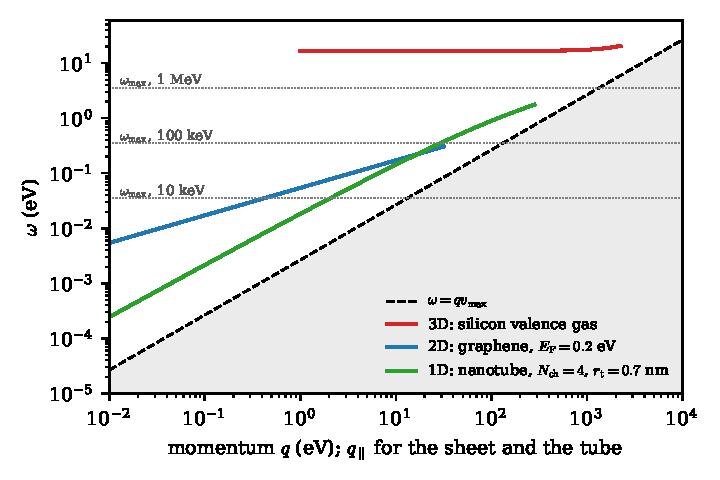
\includegraphics[width=0.85\linewidth]{figures/ch16/fig16_2.pdf}
  \caption{Plasmons in three, two and one dimensions against the reach of halo dark matter. Red: the valence-electron gas of silicon, $\omega_{\mathrm{pl}}^2 = \omega_p^2 + \tfrac35v_{\mathrm{F}}^2q^2$ with $\omega_p = \SI{16.6}{eV}$, to the quadratic cutoff at \SI{2.24}{keV}. Blue: doped graphene in vacuum at a Fermi energy of \SI{0.2}{eV}, $\omega_{\mathrm{pl}}^2 = 2\alpha E_{\mathrm{F}}q_\parallel$, up to the interband edge at \SI{32}{eV}. Green: the charge mode of a metallic nanotube, \cref{eq:16.2-wire} with $N_{\mathrm{ch}} = 4$, $r_{\mathrm{t}} = \SI{0.7}{nm}$, $\varepsilon_{\mathrm{env}} = 1$ and $v_{\mathrm{D}} = 3.02\times10^{-3}$, to $q_\parallel = 1/r_{\mathrm{t}}$. Dashed: $\omega = qv_{\mathrm{max}}$, the largest energy a halo particle deposits with momentum $q$ (gray below it). Dotted: the largest energy $\mchi v_{\mathrm{max}}^2/2$ for three masses. The bulk mode lies above the dashed line at its own $q$ and is out of reach. The modes of the sheet and the tube depend only on $q_\parallel$, and a particle reaches them with a total momentum $q \ge \omega/v_{\mathrm{max}}$, the rest of it across the sheet or the tube.}
  \label{fig:16-dispersion}
\end{figure}

\Cref{eq:16.2-wire} rests on the linear band. A real band curves on the scale of its Fermi momentum, and the limit check below compares the linear channels with parabolic ones of the same velocity $v$ at $k_{\mathrm{F}}$, of mass $m^* = k_{\mathrm{F}}/v$. The one-dimensional Lindhard function of one such channel is $(m^*/2\pi q_\parallel)\ln[(\omega^2 - \omega_-^2)/(\omega^2 - \omega_+^2)]$, with $\omega_\pm = q_\parallel v \pm q_\parallel^2/2m^*$ the edges of its pair band, and the zero of the random-phase dielectric function has the closed form $\omega^2 = (\omega_+^2\ee^{y} - \omega_-^2)/(\ee^{y} - 1)$, with $y = 2\pi q_\parallel/(N_{\mathrm{ch}}v_{\mathrm{C}}^{\mathrm{1D}}m^*)$. Expanding it in $y$, the $q_\parallel^3$ terms cancel and the plasmon frequency is
\begin{equation*}
  \frac{\omega_{\mathrm{pl}}^{\mathrm{par}}}{\omega_{\mathrm{pl}}} = 1 + \frac{q_\parallel^2}{2k_{\mathrm{F}}^2}\,g_c^2\Bigl[\frac14 + \frac{g_c^2}{3(1 - g_c^2)}\Bigr] + O\bigl(q_\parallel^4/k_{\mathrm{F}}^4\bigr) .
\end{equation*}
The correction carries $g_c^2$: the stronger the interaction, the further the plasmon lies above the pairs, and the less the shape of the band matters. In a nanotube the linear band itself ends at the next subbands, whose pairs open at $2v_{\mathrm{D}}/r_{\mathrm{t}} = \SI{1.7}{eV}$; below that energy and for $q_\parallel \ll 1/r_{\mathrm{t}}$ the four channels are the whole low-energy response. In a forest of parallel tubes the Coulomb interaction between tubes adds to $v_{\mathrm{C}}^{\mathrm{1D}}$ once $q_\perp$ is below the inverse spacing, 1 to \SI{2}{eV} for the spacings of 100 to \SI{200}{nm} that Ref.~\cite{zhang2026luttinger} considers.

\begin{limitbox}[One-dimensional plasmons of linear channels][lim:16.2a]
$S_{\mathrm{1D}} = N_{\mathrm{ch}}g_c|q_\parallel|\delta(\omega - v|q_\parallel|/g_c)$ with $g_c = [1 + N_{\mathrm{ch}}v_{\mathrm{C}}^{\mathrm{1D}}/\pi v]^{-1/2}$; Zhang and Chen give the case $N_{\mathrm{ch}} = 1$, and a metallic nanotube has $N_{\mathrm{ch}} = 4$~\cite[Eqs.~(3)--(6)]{zhang2026luttinger}.
\par\smallskip
{\centering
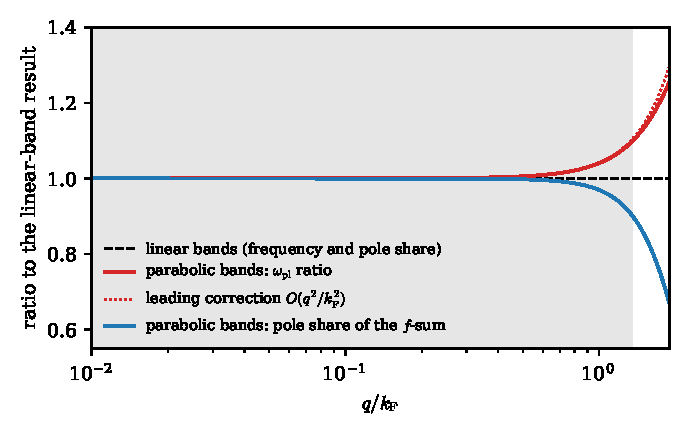
\includegraphics[width=0.82\linewidth]{figures/ch16/limit16_2a.pdf}
\captionof{figure}{Plasmon frequency and pole share of the $f$-sum for $N_{\mathrm{ch}} = 4$ parabolic channels, relative to the linear-band result, against $q_\parallel/k_{\mathrm{F}}$. Both use the kernel of a tube of radius \SI{0.7}{nm} in vacuum and the velocity $v_{\mathrm{D}} = 3.02\times10^{-3}$ at $k_{\mathrm{F}}$; the parabolic band, of mass $k_{\mathrm{F}}/v_{\mathrm{D}}$ with $k_{\mathrm{F}} = 1/r_{\mathrm{t}} = \SI{282}{eV}$, is a model for the curvature that the subbands bring on that scale. Red: frequency ratio; dotted, its leading correction in $q_\parallel^2/k_{\mathrm{F}}^2$. Blue: share of the $f$-sum $N_{\mathrm{ch}}vq_\parallel^2$ in the plasmon line (one for linear bands). Gray: both within \SI{10}{\percent} of the linear-band result, $q_\parallel < 1.36\,k_{\mathrm{F}}$. Along the curve $g_c$ rises from 0.18 to 0.61.}\label{fig:16-wire-limit}
\par}
\smallskip
Beyond $q_\parallel \approx 1.4\,k_{\mathrm{F}}$ the plasmon of curved bands moves up by more than \SI{10}{\percent} and loses weight to the pair continuum, which linear bands do not have.
\end{limitbox}

In the random-phase approximation the line of \cref{eq:16.2-wire} does not decay, and neither does the sheet plasmon above the pair continuum. Such a plasmon is a final state of its own in the sense of \cref{sec:8.7}, unlike the bulk plasmon of silicon, which decays into pairs at once. Its energy leaves the tube or sheet by propagating to the contacts, where Ref.~\cite{zhang2026luttinger} proposes to convert it into quasiparticles of a superconductor, or by damping through disorder, phonons or the substrate. How much of it reaches a sensor is a question for the cascade of \cref{chap:18}, not for the response.

\subsection{The acoustic plasmon of two components}\label{sec:16.2-demon}

A material with two kinds of carriers, light electrons of Fermi velocity $v_{\mathrm{F},l}$ and heavy ones of mass $m_h$ and density $\nd_h$, has a second collective mode below the plasmon. It is known as Pines' demon, after its prediction in 1956~\cite{pines1956electron}. In the window $qv_{\mathrm{F},h} \ll \omega \ll qv_{\mathrm{F},l}$ the light electrons follow the potential statically and screen it, while the heavy ones respond as a free plasma. Take the light response at $q \ll k_{\mathrm{F},l}$ from \cref{eq:4.5-lindhard}, $R^0_l = -2\mathcal{N}_{\mathrm{F},l}\,f_3(\nu)$ with $\nu = \omega/qv_{\mathrm{F},l}$ and $f_3(\nu) = 1 - (\nu/2)\ln|(1 + \nu)/(1 - \nu)| + \ii(\pi/2)\nu\,\Theta(1 - \nu)$, and the heavy response at high frequency, $\nd_hq^2/m_h\omega^2$. In three dimensions
\begin{gather}
  \varepsilon(q,\omega) = 1 + \frac{k_{\mathrm{TF},l}^2}{q^2}\,f_3(\nu) - \frac{\omega_{p,h}^2}{\omega^2} , \notag \\
  \omega_a(q) = \frac{\omega_{p,h}\,q}{\bigl(q^2 + k_{\mathrm{TF},l}^2\bigr)^{1/2}} \simeq v_aq ,
  \qquad
  v_a = \frac{\omega_{p,h}}{k_{\mathrm{TF},l}} = \Bigl(\frac{\nd_h}{2m_h\mathcal{N}_{\mathrm{F},l}}\Bigr)^{1/2} ,
  \label{eq:16.2-demon}
\end{gather}
with $k_{\mathrm{TF},l}^2 = 2e^2\mathcal{N}_{\mathrm{F},l}$ and $\omega_{p,h}^2 = e^2\nd_h/m_h$, where $\omega_a$ is the zero of $\varepsilon$ with $\Real f_3 \simeq 1$. The heavy plasma would oscillate at $\omega_{p,h}$; the light electrons move against it and cancel its charge to within a fraction $q^2/k_{\mathrm{TF},l}^2$, and the frequency of the screened oscillation vanishes linearly in $q$. The mode is consistent if $v_{\mathrm{F},h} \ll v_a \ll v_{\mathrm{F},l}$.

Since its charge is screened, the mode carries little weight in the loss function. Near the zero, $\partial\varepsilon/\partial\omega = 2(1 + k_{\mathrm{TF},l}^2/q^2)/\omega_a$, and the line in $L = \Imag(-1/\varepsilon)$ has weight $\pi/(\partial\varepsilon/\partial\omega)$, as in \cref{eq:4.5-plasmonL}. Its first moment, compared with the $f$-sum $(\pi/2)\omega_{p,h}^2$ of the heavy carriers,
\begin{equation}
  \frac{\omega_a\cdot\pi/(\partial\varepsilon/\partial\omega)}{(\pi/2)\,\omega_{p,h}^2} = \Bigl(\frac{q^2}{q^2 + k_{\mathrm{TF},l}^2}\Bigr)^2 \quad (\text{3D}) ,
  \qquad
  \Bigl(\frac{q_\parallel}{q_\parallel + q_s}\Bigr)^2 \quad (\text{2D}) ,
  \label{eq:16.2-share}
\end{equation}
where the two-dimensional form follows below. A density coupling acts on light and heavy electrons with the same sign, and it sees the acoustic plasmon only at order $q^4/k_{\mathrm{TF},l}^4$. The mode is neutral at long wavelength, as Hochberg, Novko, Ovadia and Politano note for the demon of Sr$_2$RuO$_4$, observed there by electron energy-loss spectroscopy~\cite{hochberg2025unconventional}. Their first-principles loss function of that layered metal shows the mode along the stacking axis as a broad peak from 80 to \SI{800}{meV}, while the plasmon at \SI{1.6}{eV} dominates in the plane. Their rate is \cref{eq:4.4-SL} inserted in \cref{eq:8.2-spectrum}~\cite[Eqs.~(1), (2)]{hochberg2025unconventional}. \Cref{eq:16.2-demon,eq:16.2-share} are the two-component random-phase limit of such a loss function, which a calculation of the full crystal contains automatically. Hole-doped diamond, in the same work, has an acoustic plasmon near \SI{200}{meV} from the oscillation of its valence manifold.

The light electrons also damp the mode, since at $\omega_a < qv_{\mathrm{F},l}$ the acoustic plasmon lies inside their pair continuum. With $\Imag\varepsilon = (k_{\mathrm{TF},l}^2/q^2)(\pi/2)\nu$ and the slope above, the full width at half maximum, $\varGamma_a = 2\Imag\varepsilon/(\partial\varepsilon/\partial\omega)$, is at $q \ll k_{\mathrm{TF},l}$
\begin{equation}
  \frac{\varGamma_a}{\omega_a} = \frac{\pi}{2}\,\frac{v_a}{v_{\mathrm{F},l}} \quad (\text{3D}) ,
  \qquad
  \frac{\varGamma_a}{\omega_a} = \frac{v_a/v_{\mathrm{F},l}}{\bigl(1 - v_a^2/v_{\mathrm{F},l}^2\bigr)^{1/2}} \quad (\text{2D}) .
  \label{eq:16.2-width}
\end{equation}
The mode is well defined only while $v_a \ll v_{\mathrm{F},l}$, and the condition that made the light electrons static is the same that keeps the mode narrow. In two dimensions every step repeats with the kernel of \cref{eq:16.2-kernel2D}. The static light response gives $v_{\mathrm{C}}^{\mathrm{2D}}\cdot2\mathcal{N}_{\mathrm{F},l} = q_s/q_\parallel$, with the two-dimensional screening wavevector $q_s = 2e^2\mathcal{N}_{\mathrm{F},l}/(\varepsilon_a + \varepsilon_b)$, and the heavy plasma gives $\omega_{\mathrm{2D},h}^2 = e^2\nd_{\mathrm{2D},h}q_\parallel/[(\varepsilon_a + \varepsilon_b)m_h]$. The zero is $\omega_a^2 = \omega_{\mathrm{2D},h}^2/(1 + q_s/q_\parallel) \simeq v_a^2q_\parallel^2$, with the same $v_a = (\nd_{\mathrm{2D},h}/2m_h\mathcal{N}_{\mathrm{F},l})^{1/2}$: the charge cancels from the velocity, which depends on neither the dimension nor the substrate. The width differs. At $q_\parallel \ll k_{\mathrm{F},l}$ the two-dimensional Lindhard function below the continuum edge has $\Real f_2 = 1$ exactly and $\Imag f_2 = \nu/(1 - \nu^2)^{1/2}$, which gives the second form of \cref{eq:16.2-width}, without the factor $\pi/2$ and with no shift of the line.

\begin{limitbox}[Acoustic plasmon of two components and its Landau width][lim:16.2b]
$\varGamma_a/\omega_a = (\pi/2)v_a/v_{\mathrm{F},l}$ for the demon of a three-dimensional two-component metal~\cite{pines1956electron}, with $v_a = \omega_{p,h}/k_{\mathrm{TF},l}$ from \cref{eq:16.2-demon} and the loss function entering the rate as in Ref.~\cite[Eqs.~(1), (2)]{hochberg2025unconventional}; $(v_a/v_{\mathrm{F},l})(1 - v_a^2/v_{\mathrm{F},l}^2)^{-1/2}$ for a sheet, from the two-dimensional Lindhard response of the light carriers, \cref{eq:16.2-width}.
\par\smallskip
{\centering
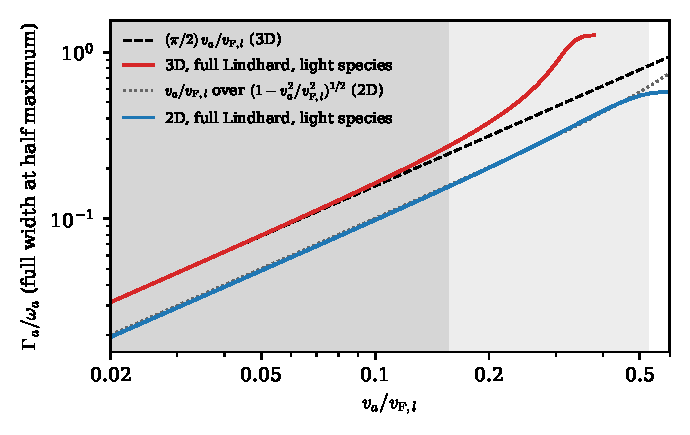
\includegraphics[width=0.82\linewidth]{figures/ch16/limit16_2b.pdf}
\captionof{figure}{Full width at half maximum of the acoustic plasmon over its frequency, against $v_a/v_{\mathrm{F},l}$. Dashed and dotted: \cref{eq:16.2-width} in three and two dimensions. Red and blue: the width of the line in $L = \Imag(-1/\varepsilon)$ with the full frequency dependence of the light carriers' Lindhard function at $q \ll k_{\mathrm{F},l}$. The heavy carriers are cold, and $q = 0.02\,k_{\mathrm{TF},l}$ (3D) and $q_\parallel = 0.02\,q_s$ (2D); the 3D curve stops at $v_a/v_{\mathrm{F},l} = 0.4$, beyond which the line is too broad and asymmetric for a width to be defined. Dark gray: the 3D form within \SI{10}{\percent}, $v_a/v_{\mathrm{F},l} < 0.157$; light gray: the 2D form within \SI{10}{\percent}, $v_a/v_{\mathrm{F},l} < 0.53$. At $v_a/v_{\mathrm{F},l} = 0.02$ the 2D width is \SI{3}{\percent} below its formula because of the finite $q_\parallel/q_s$.}\label{fig:16-demon-limit}
\par}
\smallskip
Beyond the shaded region the light carriers no longer screen statically, the line broadens into their continuum, in three dimensions with a long tail toward high frequency, and the width stops being a small correction to a sharp mode.
\end{limitbox}

\begin{workedexample}{The acoustic plasmon of a two-band sheet}\label{we:16-demon}
Take a sheet suspended in vacuum with two parabolic, spin-degenerate bands of areal density $\nd_{\mathrm{2D}} = \SI{1.0e13}{cm^{-2}}$ each, and masses $m_l = 0.2\,m_e$ and $m_h = 4.0\,m_e$, model values chosen to show the mode. Both bands have $k_{\mathrm{F}} = (2\pi\nd_{\mathrm{2D}})^{1/2} = \SI{156.4}{eV}$ (\SI{0.793}{nm^{-1}}), so $v_{\mathrm{F},l} = 1.53\times10^{-3}$ and $v_{\mathrm{F},h} = 7.65\times10^{-5}$. With $2\mathcal{N}_{\mathrm{F},l} = m_l/\pi$, the screening wavevector is $q_s = e^2m_l/2\pi = 2\alpha m_l = \SI{1.49}{keV}$.

\emph{Velocity.} $v_a^2 = \nd_{\mathrm{2D}}\pi/(m_hm_l) = k_{\mathrm{F}}^2/(2m_hm_l)$, so $v_a = 2.42\times10^{-4}$, or \SI{72.5}{km.s^{-1}}. The mode lies between the continua: $v_a/v_{\mathrm{F},l} = (m_l/2m_h)^{1/2} = 0.158$ and $v_a/v_{\mathrm{F},h} = 3.16$.

\emph{Frequency and width at $q_\parallel = \SI{20}{eV}$.} Here $q_\parallel/k_{\mathrm{F}} = 0.128$ and $q_\parallel/q_s = 0.0134$. The heavy band alone would oscillate at $\omega_{\mathrm{2D},h} = \SI{41.8}{meV}$; screened, $\omega_a = \omega_{\mathrm{2D},h}(1 + q_s/q_\parallel)^{-1/2} = \SI{4.81}{meV}$. \Cref{eq:16.2-width} gives $\varGamma_a/\omega_a = 0.160$, a width of \SI{0.77}{meV}. Both bands together carry the ordinary sheet plasmon at \SI{191.5}{meV} to leading order (\SI{193}{meV} with the $v_{\mathrm{F}}^2$ term of \cref{eq:16.2-2Dpl}), far above $q_\parallel v_{\mathrm{F},l} = \SI{30.6}{meV}$.

\emph{Weight.} By \cref{eq:16.2-share} the line carries $(q_\parallel/(q_\parallel + q_s))^2 = 1.75\times10^{-4}$ of the heavy band's $f$-sum. The light band's own pair continuum carries about as much in the lower half of its range, below $\tfrac12q_\parallel v_{\mathrm{F},l} = \SI{15.3}{meV}$: $1.72\times10^{-4}$ of the same sum, spread over all energies up to there.

\emph{Check.} Now treat both bands with the two-dimensional Lindhard function at $q_\parallel \ll k_{\mathrm{F}}$, so that the heavy band is no longer assumed cold. The peak of $L$ then sits at \SI{4.97}{meV} with a width of \SI{0.76}{meV} ($\varGamma_a/\omega_a = 0.154$), and the first moment within three widths of the peak is $1.76\times10^{-4}$ of the heavy $f$-sum. The heavy band raises the frequency by \SI{3.5}{\percent}, the size of $\tfrac34(v_{\mathrm{F},h}/v_a)^2 = 0.075$ in $\omega_a^2$.

\emph{Kinematics.} A halo particle deposits \SI{4.81}{meV} if $\mchi \ge 2\omega_a/v_{\mathrm{max}}^2 = \SI{1.37}{keV}$, and supplies $q_\parallel = \SI{20}{eV}$ if $2\mchi v_{\mathrm{max}} \ge \SI{20}{eV}$, or $\mchi \ge \SI{3.8}{keV}$. The energy needs a total momentum of only $\omega_a/v_{\mathrm{max}} = \SI{1.8}{eV}$, and the in-plane \SI{20}{eV} decides. The mode, eleven times slower than the fastest halo particles, is reachable by keV-mass dark matter. Its weight, however, is four orders of magnitude below that of the heavy band: a density coupling scatters off this sheet mostly through the pair continuum and the optical plasmon, not through the acoustic one.
\end{workedexample}

\subsection{Layered stacks}\label{sec:16.2-stacks}

A stack of identical sheets with period $a_s$ in a background $\varepsilon_b$, with no tunneling between them, is the simplest layered target. The sheets interact, and \cref{eq:16.2-embed} no longer applies. A density wave $\delta\nd_{\mathrm{2D}}\,\ee^{\ii\vect{q}_\parallel\cdot\vect{r}_\parallel}$ on sheet $n$, with the phase $\ee^{\ii q_zna_s}$ of the external potential, produces $(e^2/2\varepsilon_bq_\parallel)\ee^{-q_\parallel|z - na_s|}$ at height $z$, and the sum over sheets at $z = 0$ is a geometric series. Each sheet therefore sees the kernel
\begin{gather}
  v_{\mathrm{C}}^{\mathrm{L}}(q_\parallel,q_z) = \frac{e^2}{2\varepsilon_bq_\parallel}\sum_n\ee^{-q_\parallel|n|a_s + \ii q_zna_s} = \frac{e^2}{2\varepsilon_bq_\parallel}\,\frac{\sinh q_\parallel a_s}{\cosh q_\parallel a_s - \cos q_za_s} , \notag \\
  S(\vect{q},\omega) = -\frac{2}{a_s}\,\Imag\frac{\tilde R^{\mathrm{2D}}}{1 - v_{\mathrm{C}}^{\mathrm{L}}\tilde R^{\mathrm{2D}}} ,
  \label{eq:16.2-sheets}
\end{gather}
at $T = 0$, per unit volume, for sheets thinner than $1/q$, with the background treated as a static dielectric. For $a_s \to \infty$ the kernel becomes that of an isolated sheet, and $S$ is $1/a_s$ times its structure factor. For $q_\parallel a_s, q_za_s \ll 1$ it becomes $e^2/(\varepsilon_ba_sq^2)$, the bulk kernel acting on the density $\nd_{\mathrm{2D}}/a_s$. In between, the stack carries a band of layer plasmons. For parabolic sheets, $\omega^2 = v_{\mathrm{C}}^{\mathrm{L}}\nd_{\mathrm{2D}}q_\parallel^2/m^*$ runs at small $q_\parallel$ from the bulk plasma frequency of the density $\nd_{\mathrm{2D}}/a_s$ at $q_z = 0$, where all sheets oscillate in phase, down to the acoustic mode $\omega^2 = e^2\nd_{\mathrm{2D}}a_sq_\parallel^2/4\varepsilon_bm^*$ at $q_za_s = \pi$, where neighbors oscillate against each other. The dark-matter momentum along the axis is not reduced to a zone, since the sheets have no structure on the scale of $1/q$; $S$ is periodic in $q_z$ with period $2\pi/a_s$ until the profile of a sheet cuts it off.

Layers many atoms thick respond through their own local dielectric functions. Take layers of materials A and B, of thicknesses $d_A$ and $d_B = a_s - d_A$, filling $f = d_A/a_s$, and local dielectric functions $\varepsilon_A(\omega)$, $\varepsilon_B(\omega)$. When the wavelength is long compared with $a_s$, the field within one period is that of a uniform field across planar boundaries. The tangential field is continuous, so the in-plane displacement is the volume average of $\varepsilon$; the normal displacement is continuous, so the normal field is the volume average of $1/\varepsilon$. The stack is a uniaxial medium with its optic axis along the stacking direction, and with $\theta$ the angle between $\vect{k}$ and that axis,
\begin{gather}
  \varepsilon_\perp = f\varepsilon_A + (1 - f)\,\varepsilon_B , \qquad
  \frac{1}{\varepsilon_\parallel} = \frac{f}{\varepsilon_A} + \frac{1 - f}{\varepsilon_B} , \notag \\
  L(\vect{k},\omega) = \Imag\frac{-1}{\varepsilon_\parallel\cos^2\theta + \varepsilon_\perp\sin^2\theta} \qquad (ka_s \to 0) .
  \label{eq:16.2-emt}
\end{gather}
Since $\varepsilon_\parallel = \varepsilon_A\varepsilon_B/[(1 - f)\varepsilon_A + f\varepsilon_B]$ and $\varepsilon_\perp[(1 - f)\varepsilon_A + f\varepsilon_B] = \varepsilon_A\varepsilon_B + f(1 - f)(\varepsilon_A - \varepsilon_B)^2$, the inverse $1/(\varepsilon_\parallel\cos^2\theta + \varepsilon_\perp\sin^2\theta)$ equals $[(1 - f)\varepsilon_A + f\varepsilon_B]/[\varepsilon_A\varepsilon_B + f(1 - f)(\varepsilon_A - \varepsilon_B)^2\sin^2\theta]$. This is identical, at every filling, to the effective longitudinal response of Lasenby and Prabhu~\cite[Eq.~(16)]{lasenby2022dark}, which they state for $d_A/a_s \ll 1$. The loss function has one line in each direction, at the zero of the denominator. For metal layers in vacuum the line falls toward zero frequency as $\vect{k}$ approaches the axis: with $\varepsilon_A = \varepsilon_\infty(1 - \omega_p^2/\omega^2)$ and small $\theta$ and $f$ it sits at $\omega^2 \simeq f\varepsilon_\infty\omega_p^2\theta^2/\varepsilon_B$, the filling fraction times the plasma frequency squared, reduced by the direction~\cite{lasenby2022dark}.

For $\vect{k}$ in the plane of the layers the response is known in closed form at every $ka_s$. The source $\ee^{\ii kz}$ is uniform across the layers, and the potential is $\psi(x)\ee^{\ii kz}$ with $x$ along the axis. Inside layer $j$ it is the particular solution $1/\varepsilon_jk^2$ plus $C_j\cosh[k(x - x_j)]$, symmetric about the center $x_j$ of the layer. Continuity of $\psi$ and of $\varepsilon\,\partial_x\psi$ at an interface fixes $C_A = (\varepsilon_A - \varepsilon_B)s_B/[k^2\varepsilon_A(\varepsilon_Bs_Bc_A + \varepsilon_As_Ac_B)]$ and $C_B = -\varepsilon_As_AC_A/\varepsilon_Bs_B$, with $s_j = \sinh(kd_j/2)$ and $c_j = \cosh(kd_j/2)$. The average of $k^2\psi$ over a period is the head of $\varepsilon^{-1}$ at the external wavevector:
\begin{keyresult}[Stack of two dielectrics, $\vect{k}$ in the plane]
\begin{equation}
  \frac{1}{\varepsilon(k,\omega)} = \frac{f}{\varepsilon_A} + \frac{1 - f}{\varepsilon_B} - \frac{2}{ka_s}\,\frac{(\varepsilon_A - \varepsilon_B)^2\,s_As_B}{\varepsilon_A\varepsilon_B\,(\varepsilon_As_Ac_B + \varepsilon_Bs_Bc_A)} ,
  \label{eq:16.2-inplane}
\end{equation}
with $L = \Imag[-1/\varepsilon]$, exact for local $\varepsilon_A$, $\varepsilon_B$ at any $ka_s$.
\end{keyresult}
\noindent At $ka_s \to 0$, $s_j \to kd_j/2$, $c_j \to 1$, and the right side becomes $1/\varepsilon_\perp$, the in-plane limit of \cref{eq:16.2-emt}. Expanding to the next order,
\begin{equation}
  \frac{1}{\varepsilon(k,\omega)} = \frac{1}{\varepsilon_\perp} + (ka_s)^2\,\frac{f^2(1 - f)^2(\varepsilon_A - \varepsilon_B)^2}{12\,\varepsilon_\parallel\,\varepsilon_\perp^2} + O\bigl((ka_s)^4\bigr) .
  \label{eq:16.2-corr}
\end{equation}
The correction is quadratic in the period over the wavelength and grows with the contrast between the layers. At $ka_s \to \infty$, $s_j/c_j \to 1$ and the response is the volume average of $1/\varepsilon_j$: each layer then screens as its own bulk. One layer alone follows for $d_B \to \infty$ with $\varepsilon_B = 1$. Multiplied by $a_s$, $\varepsilon^{-1} - 1$ becomes the response per unit area, $d_A(1/\varepsilon_A - 1) - 2(\varepsilon_A - 1)^2s_A/[k\varepsilon_A(\varepsilon_As_A + c_A)]$, and minus this equals the thin-film response of Lasenby and Prabhu up to the real constant $d_A$, which does not enter the loss~\cite[Eq.~(19)]{lasenby2022dark}: the constant is the vacuum term that their response, normalized to $-d/\varepsilon$ for a bulk slab, does not subtract. Its line sits at $\varepsilon_A = -\coth(kd_A/2)$; for a Drude metal at $kd_A \ll 1$ that is $\omega^2 = \omega_p^2kd_A/2$, the sheet plasmon of \cref{eq:16.2-2Dpl} with $\nd_{\mathrm{2D}} = \nd_ed_A$ in vacuum. With $|\varepsilon_A| \gg 1$ and $kd_A \ll 1$ the same expression reduces to the sheet screening of \cref{eq:15.3-sheet}. For a general direction the same matching, with the Bloch condition $\psi(x + a_s) = \ee^{\ii k_xa_s}\psi(x)$ across one period, gives $\varepsilon^{-1}$ by solving four linear equations; it also approaches \cref{eq:16.2-emt} at small $ka_s$.

\begin{limitbox}[Effective medium of a layered stack][lim:16.2c]
For $ka_s \to 0$ a stack of layers with local $\varepsilon_A$, $\varepsilon_B$ and filling $f$ has $1/\varepsilon_L = [(1 - f)\varepsilon_A + f\varepsilon_B]/[\varepsilon_A\varepsilon_B + f(1 - f)(\varepsilon_A - \varepsilon_B)^2\sin^2\theta]$, $\theta$ measured from the stacking axis~\cite[Eq.~(16)]{lasenby2022dark}.
\par\smallskip
{\centering
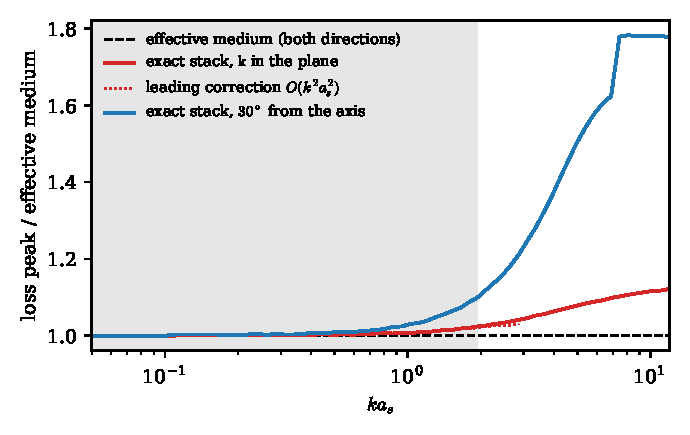
\includegraphics[width=0.82\linewidth]{figures/ch16/limit16_2c.pdf}
\captionof{figure}{Frequency of the loss peak of a model stack relative to the effective medium, against $ka_s$. Layers of \SI{1}{nm} with $\varepsilon_A = 10[1 - \omega_p^2/\omega(\omega + \ii\gamma)]$, $\omega_p = \SI{0.5}{eV}$, $\gamma = 0.1\,\omega_p$, alternate with \SI{4}{nm} of vacuum ($a_s = \SI{5}{nm}$, $f = 0.2$), the toy stack of Lasenby and Prabhu. Red: $\vect{k}$ in the plane, exact (\cref{eq:16.2-inplane}); dotted, the leading correction \cref{eq:16.2-corr}. Blue: $\vect{k}$ at \SI{30}{\degree} from the axis, exact solution of the periodic stack. The effective-medium peaks are at 0.4215 and \SI{0.2740}{eV}. Gray: both within \SI{10}{\percent} of the effective medium, $ka_s < 1.94$. At $ka_s = 12$ the peaks are at 0.473 and \SI{0.487}{eV}, near the surface plasmon of a single layer, $\varepsilon_A = -\varepsilon_B$ (\SI{0.477}{eV} without damping).}\label{fig:16-stack-limit}
\par}
\smallskip
Beyond $ka_s \approx 2$ the field varies within a period, the line of an oblique direction moves up by tens of percent toward that of a single layer, and the stack must be treated layer by layer.
\end{limitbox}

A single undamped line in each direction is the case in which the sum-rule bound of \cref{sec:10.2} can be reached. For $L = A\,\delta(\omega - \omega_{\vect{k}})$ every moment is $K_n = A\omega_{\vect{k}}^n$, and the Hölder inequality behind \cref{eq:10.2-Kn} holds as an equality; the bound \cref{eq:10.2-bound} is then attained when the line sits where $\omega^{-n}\eta$ is largest. A bulk metal places its line at $\omega_p$, far above what light dark matter deposits. A stack moves it down by the filling fraction and the direction, which is why Lasenby and Prabhu proposed it~\cite{lasenby2022dark}. For the model stack of the limit check, \SI{10}{\percent} accuracy at \SI{30}{\degree} ends at $k = \SI{77}{eV}$, the largest momentum transfer, $2\mchi v_{\mathrm{max}}$, of a particle of \SI{14.5}{keV}. Heavier dark matter probes the stack at momenta where the field varies within a period, and needs the full periodic response, with $q_z$ unreduced, that \cref{app:E.21} specifies, and at $k \gtrsim 1/d_A$ also the nonlocal response $\varepsilon_A(\vect{k},\omega)$ of the layer material itself.
